\chapter{Results}
\label{res}

\section{The first set of physicochemical attributes}
\label{res:first}

	In this section, results for the first set of physicochemical properties described
	above will be presented.
	These include the length, pI, GRAVY index, and percentage of charged amino acids within
	the inter-domain regions of human two-domain PKs containing one PK domain.

	\subsection{Feature distributions (densities)}
	\label{res:first:dens}

		The density analysis gave interesting insights into the distribution of
		physicochemical properties within the studied dataset.
		The linker length density peaks around 75 residues.
		A small portion of extremely long inter-domain regions spanning 500 to 800 residues is
		also present.
		However, it is questionable, whether these ``linkers'' might not represent a yet
		unrecognized domain, and thus not being suitable for the definition of a
		linker~\cite{milano2016structural}.

		A nontrivial outcome has been observed while studying the density of linkers' pI,
		visualized in \cref{fig:iso-dens}.
		Most non-domain regions in human two-domain PKs are either very acidic, or, on the
		other hand, very basic.
		Interestingly, the region of a neutral pH contains almost no proteins, forming an
		empty gap around pH 8.
		This allows for dividing the studied PKs into two groups based on their linker's
		acidity.

		\begin{figure}
			\centering
			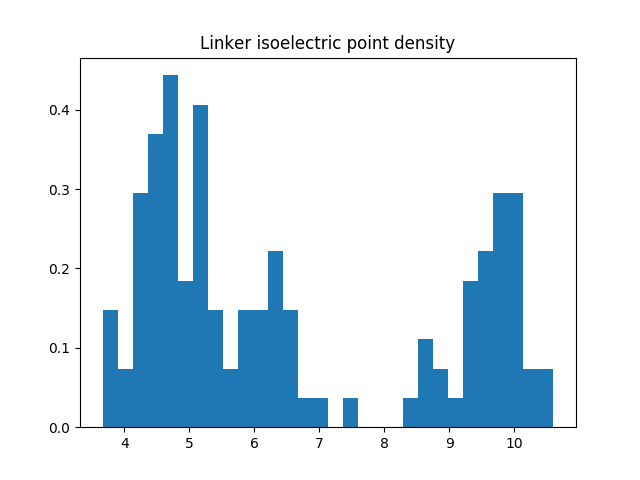
\includegraphics[width=.7\linewidth]{img/iso_density.png}
			\caption{The pI density of inter-domain regions from human two-domain PKs in the
			studied dataset.
			Two groups of proteins are evident, one with acidic linkers, one with basic
			linkers.}
			\label{fig:iso-dens}
		\end{figure}

		Au contraire, neither the percentage of charged amino acids within the inter-domain
		regions nor the linkers' GRAVY index form distinct clusters.
		Their densities show only single local maxima.
		All linkers from the final dataset are hydrophilic; the fraction of charged residues
		averages around 0.25.

	\subsection{UMAP dimensionality reduction}
	\label{res:first:umap}

		Three clusters corresponding to three distinct linker types were identified visually
		in the UMAP projection of the first set of the linkers' physicochemical attributes.
		Throughout this thesis, the linker types will be referred to based on the clusters'
		positioning in \cref{fig:umap}: ``L-linkers'' for the lower left cluster,
		``M-linkers'' for the middle cluster, and ``R-linkers'' for the right cluster.
		L-linkers are best characterized by their extreme length of more than 600 residues,
		R-linkers by their extremely basic pI, and M-linkers by their extremely acidic pI.

		\begin{figure}
			\centering
			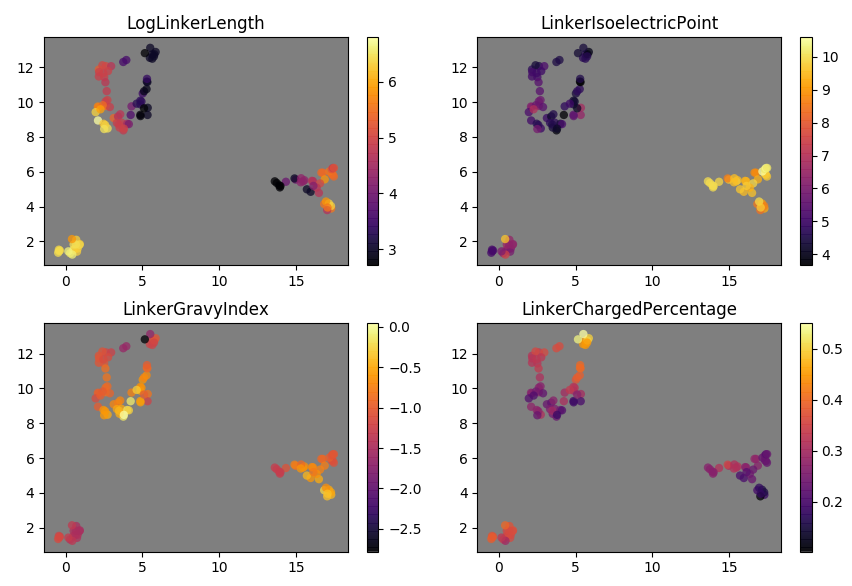
\includegraphics[width=\linewidth]{img/linker_umap.png}
			\caption{The UMAP dimensionality reduction on the normalized linker attributes:
			logarithm of the linker's length, its pI, its GRAVY index, and
			a percentage of charged amino acids within the inter-domain regions of human
			two-domain PKs.
			Each subfigure presents the distribution of the values of the respective property.}
			\label{fig:umap}
		\end{figure}

		\begin{figure}
			\centering
			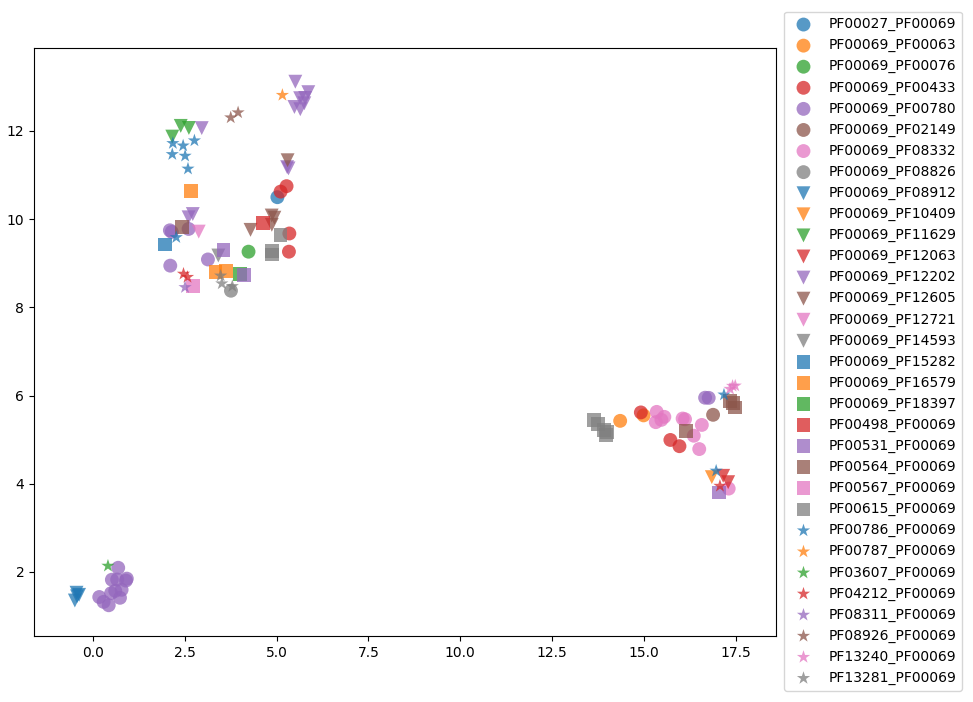
\includegraphics[width=\linewidth]{img/linker_umap_arch.png}
			\caption{Architectures of the studied molecules embedded into the UMAP projection
			of the four physicochemical attributes of the inter-domain regions.}
			\label{fig:umap_arch}
		\end{figure}

		By embedding the architectures of the proteins from the studied dataset into the UMAP
		representation it became visible that many architectures feature more than one linker
		type, as seen in \cref{fig:umap_arch}.
		Especially, the architecture \texttt{PF00069\_PF00780} stands out, being endowed with
		all three linker classes.
		On the other hand, most architectures equipped with linkers from only one category
		are represented by a very small subset of proteins from the set of human two-domain
		PKs.

	\subsection{Gene Ontology terms}
	\label{res:first:go}

		All considered proteins had at least two GO terms assigned, one of them being always
		\texttt{GO:0005524; F:ATP binding}.
		The second most common GO term was \texttt{GO:0004674; F:protein serine/threonine
		kinase activity}, and the third most frequent GO term was \texttt{GO:0004672;
		F:protein kinase activity}.

		However, the search for unique GO terms within both the UMAP representation and the pI
		clustering of the non-domain regions on different GO hierarchical levels gave no
		satisfactory results, albeit discovering many GO terms exclusive for each examined
		linker group.
		Unfortunately, the numbers of proteins carrying these terms were too low to permit a
		robust analysis.
		No single GO terms were identified which would be associated exclusively with all members of individual clusters.

		There were only two GO terms standing out regarding their proportion.
		\texttt{GO:0000287; F:magnesium ion binding} found on hierarchy level 6 is exclusive
		to the acidic linker group, as well as to the M-linkers.
		It was encountered in 12 proteins covering 8 different architectures, including those
		having the PK domain on the N-terminus, as well as those carrying the PK domain on the
		C-terminus.
		The second vocable is \texttt{GO:0005516; F:calmodulin binding}, appearing on the
		hierarchy level 4.
		This term is limited to the basic linker group and to the R-linkers.
		In this case, all 10 proteins accredited with this GO term possess the same
		architecture.

	\subsection{Enzyme Commission numbers}
	\label{res:first:ec}

		\begin{figure}
			\centering
			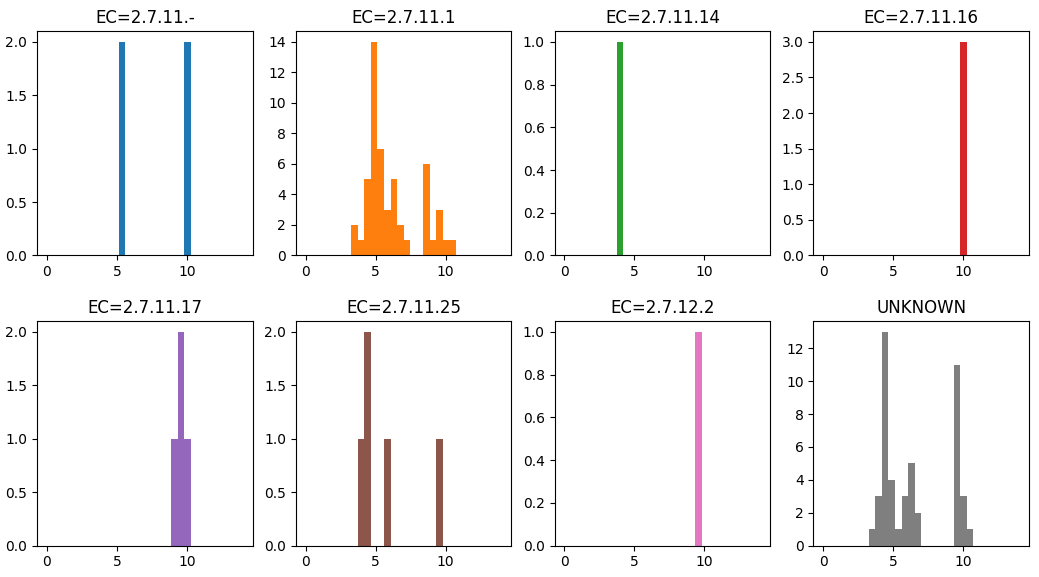
\includegraphics[width=\linewidth]{img/iso_density_ec.png}
			\caption{Occurrences of EC numbers in human two-domain PKs.
			The $x$-axis represents the pI of the molecules' linkers.}
			\label{fig:ec}
		\end{figure}

		Out of the 117 human two-domain PKs, 70 molecules have an EC number assigned in the
		URP.dat file.
		For the remaining 47, the EC term will be reffered to as ``\texttt{UNKNOWN}''.
		3 kinases had more than one EC number specified; some of these extra terms are
		outside of the \texttt{2.7.11 protein-serine/threonine kinases} group.
		Only 14 molecules had, however, EC classification other than \texttt{2.7.11.-},
		\texttt{2.7.11.1 non-specific serine/threonine protein kinase}, or \texttt{UNKNOWN}.

		\Cref{fig:ec} shows the distribution of the linkers' pI for each EC number.
		All 5 specialized EC terms are vastly underrepresented within the studied dataset,
		yet, for example, the \texttt{2.7.11.25 mitogen-activated protein kinase kinase
		kinases} are present in both acidic and basic linker clusters.
		Contrarily, basic inter-domain regions seem to be specific to both \texttt{2.7.11.16
		G-protein coupled receptor kinases} and
		\texttt{2.7.11.17 Ca\textsuperscript{2+}/calmodulin-dependent protein kinases};
		nevertheless, they are not to be found in more than one architecture.

		\begin{figure}
			\centering
			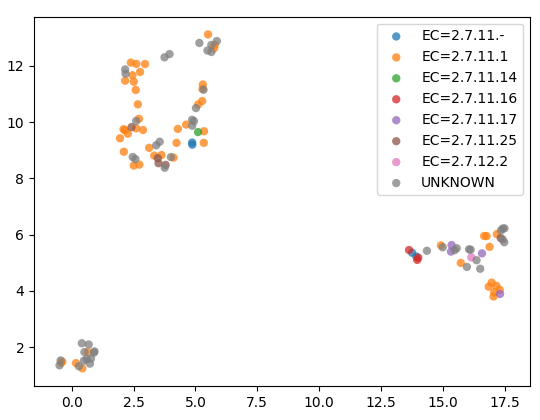
\includegraphics[width=0.8\linewidth]{img/linker_umap_ec.png}
			\caption{Embedding of the EC numbers into the UMAP representation.}
			\label{fig:umap_ec}
		\end{figure}

		The inadequate representation of the EC numbers in the final dataset was also the
		reason behind the unsatisfactory results of embedding the terms into the UMAP
		representation.
		On one hand, the numbers \texttt{2.7.11.14}, \texttt{2.7.11.16}, and
		\texttt{2.7.11.17} are specific to one of the three defined linker groups; on the
		other hand, they are not to be found in more than one architecture, as already
		mentioned above.
		In conclusion, the first set of physicochemical attributes did not provide any
		functionally relevant results.

\section[The second set of physicochemical attributes]{The second set of
physicochemical\\ attributes}
\label{res:second}

	The two-dimensional UMAP representation of the 553 physicochemical data from the AAindex
	database did not reflect the clustering of the 4 physicochemical attributes described
	above.
	As seen in \cref{fig:aa_umap}, one small cluster of inter-domain regions from human
	two-domain PKs emerges on the right side of the visualization; however, it contains only
	proteins with the same architecture \texttt{PF00069\_PF12202}.
	In the large cloud on the left side, generally, molecules with the same architecture
	create local bundles and they only seldom mix with proteins with other architectures.
	Due to the lack of clearly distinguishable clusters, no GO or EC embedding was
	performed.

	\begin{figure}
		\centering
		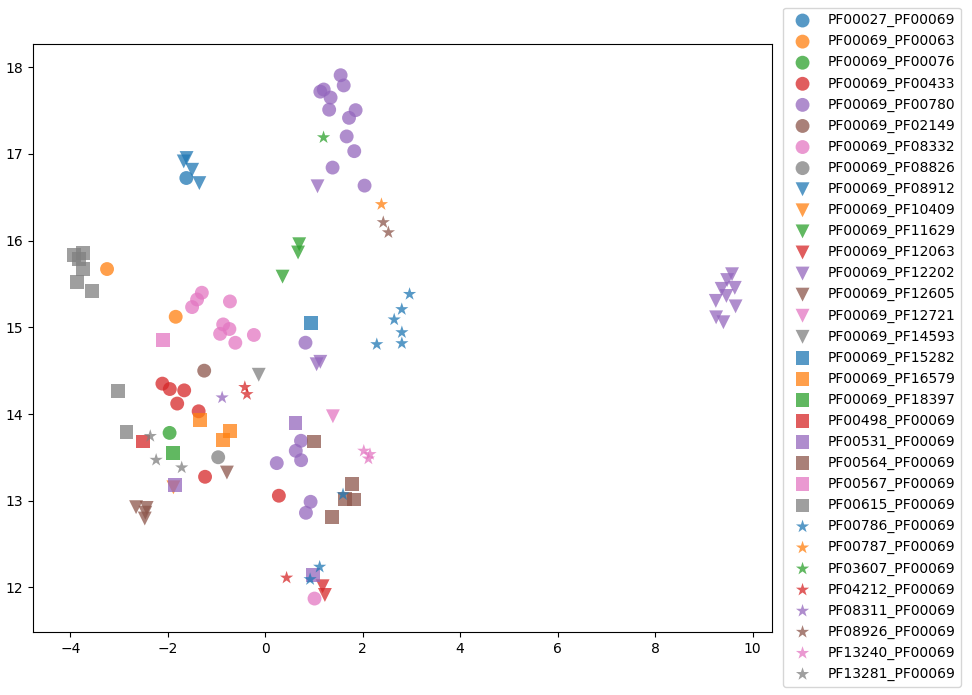
\includegraphics[width=\linewidth]{img/aa_umap_arch.png}
		\caption{Architectures of the two-domain PKs with a single PK domain embedded into the
		UMAP representation of 553 physicochemical properties from the AAindex database.}
		\label{fig:aa_umap}
	\end{figure}

	In conclusion, no obvious influence of the inter-domain regions' composition on the
	activity or specificity of human two-domain PKs with exactly one PK domain was observed,
	as no clustering of the linkers' physicochemical properties resulted in the
	colocalization of like GO or EC terms associated with proteins with different
	architectures.
